\documentclass[11pt]{article}
\usepackage{geometry}
\usepackage{graphicx}
\usepackage{array}
\usepackage{rotating}
\usepackage{pdflscape}
\usepackage{amsmath}
\numberwithin{figure}{section}
\numberwithin{table}{section}

%border spacing
\geometry{
 a4paper,
 lmargin = 1in,
 rmargin = 1in,
 tmargin = 1in,
 bmargin = 1in 
 }
 
%line spacing
\renewcommand{\baselinestretch}{1.5}  

\begin{document} 
%\begin{titlepage}
%\begin{center}
%	\vspace*{60mm}	
%	\huge
%	\textbf{   Elephant detection and localization using infra-sound waves.}
%\end{center}
%\vfill
%K K T P Ranathunga\\
%12001122

%\end{titlepage}

\begin{titlepage}
	
	\centering
	\renewcommand{\baselinestretch}{1.7}\normalsize
	
	{\fontsize{1cm}{1.2em}\selectfont \scshape Elephant detection and localization using infrasound}
	
	\vspace*{2\baselineskip}	
		

	\underline{\fontsize{0.8cm}{1.2em}\selectfont \scshape Outline of the thesis}
	\renewcommand{\baselinestretch}{1.25}\normalsize
	
	\vspace*{2\baselineskip}
	
	{by}
	
	\vspace*{0.3\baselineskip}
	{\Large K.K.T.P Ranathunga}
	\vspace*{0.3\baselineskip}
	
	{\itshape (Registration No : 2012/CS/112, Index No : 12001122)}
	
	{\normalsize tharindu.prf@gmail.com}
	
	\vspace*{2\baselineskip}
	
	\normalsize  {{Submitted in partial fulfillment}
		
		{Of the requirements of the}
		
		{B.Sc in Computer Science 4th Year Individual Project}
		
		{(SCS4124)}}
	
	\vspace*{2\baselineskip}
	
	
\includegraphics[scale=0.1]{ucsc.png}
	
	\vfill    
	
	{Supervised by}
	
	\vspace*{0.3\baselineskip}
	
	{\Large Dr. Chamath Keppitiyagama}
	

	
	%  \begin{small}
	%  {BSc (Colombo)}
	%	\end{small}   
	\vspace*{0.5\baselineskip}
	
	
	
	\vfill
	
	{University of Colombo School of Computing\\
		Colombo 7\\
		SRI LANKA}
	
	\vfill
	{November 11, 2016}
	%	\today 
	


\end{titlepage}
\pagenumbering{roman}
\section*{Singatures}
\paragraph{}
\paragraph{}
\paragraph{}
\paragraph{}
\paragraph{}
\paragraph{}
\paragraph{}

 
	\noindent\begin{tabular}{ll}
		\makebox[2.5in]{\hrulefill} & \makebox[2.5in]{\hrulefill}\\
		Supervisor & Date\\[8ex]% adds space between the two sets of signatures
		\makebox[2.5in]{\hrulefill} & \makebox[2.5in]{\hrulefill}\\
		Student & Date\\
		\end{tabular}
\newpage		
\section*{Preface}
\paragraph{}
This  document is the proposal for  the 4th Year Individual Project  for  partial  fulfillment  of  the requirements of the Degree of Bachelor of Science in Computer Science, at University of Colombo School of Computing, University of Colombo, Sri Lanka.
\paragraph{}
This proposal  provides  the  scope  and  context  of  the  project  to  be  undertaken It details  the objectives of the research,  research  questions,  background and research methodology.This  document also  provides  the project schedule, a description of anticipated results and the final products.
\paragraph{}
The intended audience of this document is the academic staff of the University Of Colombo School Of Computing and it is intended to enable them to determine whether the project should be approved as proposed, approved with modifications, or not approved.
\newpage
\tableofcontents
\newpage
\section*{Chapter 01: Introduction.}
\begin{itemize}
  \item Goal and objectives.
  \item Research question.
  \item Research question.
  \item Hypothesis.
\end{itemize}

\section*{Chapter 02 : Literature Review.}
Related works on :
\begin{itemize}
  \item Biological researches on elephant communication. 
  \item Behavior of infra sound waves.
  \item Sound localization.
  \item Signal classification.
  \item Acoustic detection of elephants.
  \item Infra sound recording devices
\end{itemize}
\section*{Chapter 03 : Design and Methodology.}
\begin{itemize}
  \item Introducing Elocate sensors.
  \item Overview of sound localization. 
  \item Comparison of localization techniques.
  \item Application of cross correlation using Elocate sensors.
  \item Feature extraction.
  \item Signal enhancement.
  \item Classification using SVM.
\end{itemize}
\section*{Chapter 04 : Implementation.}
\begin{itemize}
  \item Electronic circuit of the sensors.
  \item Noise reduction techniques.
  \item Implementation of localization.
  \item Data collection.
  \item Implementation of pre processing.
  \item Training SVM.
  \item Testing the model.
\end{itemize}
\section*{Chapter 05 : Results and Evaluation.}
\begin{itemize}
  \item Results of each experiment conducted.
  \item A comprehensive analysis on results.
\end{itemize}
\section*{Chapter 06 : Conclusion and Future Works.}
\begin{itemize}
  \item New possibilities discovered.
  \item Problems encountered.
  \item Increasing the accuracy of detection and localization.
  \item Summary
\end{itemize}
\newpage

\pagenumbering{arabic}
\section{Goal and Objective}
\paragraph{}
The world elephant population has been on the decline \cite {13} due to many reasons, among which the human elephant conflict is a major cause. Human settlements and cultivations adjoining the forest areas have resulted in the blocking of elephant migration routes and further  the presence of crops attracts wild elephants, causing damages to livelihood of humans while threatening the lives of both elephants and humans. The wildlife conservation authorities worldwide do not possess an established method to manage this situation which is non-destructive to both elephants and humans, with most authorities having to resort to brute force, often consequently aggravating the situation in the long term \cite {13}. At present, the primary solution introduced is the use of electric fences around elephant habitats to prevent elephants venturing beyond their habitat to encroach into human settlements; an expensive and potentially life threatening solution. 
\paragraph{}
The objective of this research is to implement  a cost effective solution to the human elephant conflict building on and expanding upon the previous findings of related research. Research to date has found that elephants pass various messages using infra sound frequencies and this low frequency sound waves travel a greater distance than higher frequency waves  due to high frequency waves being more easily absorbed by air molecules compared to the lower frequency waves \cite {5}. In this research, an electronic system consisting of low cost sensors that have the capability of detecting infrasound calls emitted by the elephants as well as digital signal processing techniques are combined to  identify elephant  infrasonic vocalizations to localize the sound emitting sources. Further, attempts are made to use these information in various scenarios such as prior warning system before elephants enter a cultivation and elephant herd detection among other things.

\section{Research Questions }
\paragraph{}
This research attempt to develop a method to distinguish an elephant call in a stream of sound data and to find an effective method of infrasound source localization using the phase difference of two infrasound waves captured by several sensors placed in different distances from the sound source. The research aims to answer two basic questions using a low cost sensor system consisting of off the shelf microphones capable of capturing infrasound:

\begin{enumerate}
\item How to identify an elephant call in an infrasound wave ? 
\item How to  localize a source emitting infrasound in a noisy environment ?
\end{enumerate}

\newpage
\section{Background and significance of the project}
\paragraph{}
A typical human male voice in speech fluctuates around 110 Hertz, a female's voice at around 220 Hz and a child's at around 300 Hz. Among elephants, a typical male rumble fluctuates around a minimum of 12 Hz (more than 3 octaves below a man's voice), a female's rumble at around 13 Hz and a calf's around 22 Hz \cite {1} \cite {2}. In Asian elephants, this value fluctuates between 14 Hz to 24 Hz within 10 to 25 seconds \cite {3} due to their smaller vocal cords compared to African elephants.  Elephants produce a wide range  of sounds from very low frequency rumbles to higher frequency snorts, barks, roars, cries as well as many other type of  calls. 

\paragraph{}
Audio waves below 20 Hz frequency is considered as Infrasonic waves \cite {4}. As such, elephant rumbles can be considered as infrasonic waves and these rumbles follow all the properties of infrasonic waves. A significance of infrasonic waves is that it travels further than high frequency waves. Sound is a pressure wave vibration of molecules and as a result, whenever molecules move, there is an inevitable loss of energy as heat. As a result, sound is lost by heating the medium through which it propagates. Sound wave attenuation is frequency dependent in most media.

\begin{figure}[h]
\centering
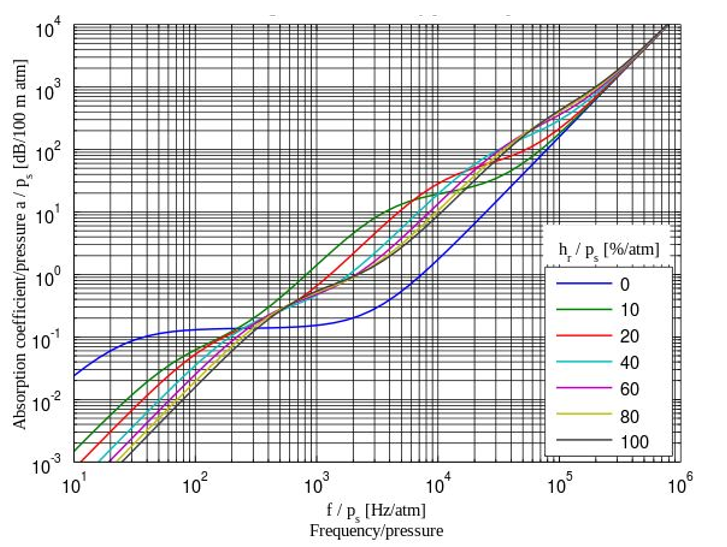
\includegraphics[width= 15cm]{a.png}
\caption{Sound absorption coefficient per atmosphere for air at 20 degree Celsius according to relative humidity per atmosphere.\cite{14}}
\label{fig:logo}
\end{figure}

\paragraph{}
The above image \ref{fig:logo} is a graph displaying the attenuation of sound at difference frequencies \cite {5}, which shows that low frequency waves have low absorption coefficient. Therefore, low frequencies are not absorbed well and travel further than high frequencies. This property of infrasound waves can be used  for the acoustic detection of the wave from a greater distance from the source of the sound. The low-frequency sounds used by elephants for long-range communication travel a distance that exceeds 1 km \cite {3}. As mentioned in the objectives, this research focusses on detecting elephant infrasonic calls from long distance and localizing them. Detecting and localizing elephants is an essential component of any viable solution to human elephant conflict. Attempts towards acoustic detection and localization of elephants exist in literature. However, due to high cost in infrasonic sensors and complexity in detection of these signals  in noisy environment, no system exists to date, that operation ready in the field.

\paragraph{}
Various types of devices which are capable of capturing infrasonic waves exist and they were mostly used for detecting geographical phenomena such as earthquakes and volcanic eruptions. One such device used by most related research is Infitec Infra 20, which has a sampling rate of 50Hz. This device can be considered as a low cost infra sound recorder compared to other existing devices and this costs US\$ 345 \cite {7}. A significance of the research is the attempt to use a laboratory made sensor system which cost only US\$ 15, which is capable of recording at a sampling rate of 44100 Hz. This sensor system consists of a Panasonic Omnidirectional Back Electret Condenser Microphone \cite{15} (Model WM-64C/WM-64K), LM358 IC for amplifying and a low pass filter\cite{16}.This sensor has the ability to capture infrasonic waves from a lower bound of 0 Hz to an approximate upper bound of 150 Hz.


\paragraph{}
The second research question is based on infrasound localization, which can be done by measuring physical quantities like sound pressure and particle velocity. The best localization technique which is used by nature (Animal sound localization) can be applied to this context in localizing a sound source digitally. Humans as well as most other land-living vertebrates use the time delay between the arrival of a sound wave at each ear to discern the direction of the source \cite {8}. Similarly, localization can be done digitally by calculating the inter-aural time delay  between two microphones lying on a specified distance, which will be further explained in the research methodology. Potential problems include the detection in noisy environment, sparsity and irregularity of elephant call and pattern recognition. These problems will be addressed using advanced digital signal processing techniques and the knowledge based on the existing literature.


\section{Literature Review}
\paragraph{}
Various research types exist in this particular domain. The experiments carried out by Katharine Payne who is a researcher in the Bioacoustics Research Program at the Laboratory of Ornithology at Cornell University show that elephants use infrasound in communication, which can be considered as the initial steps of all research work on this subject. In 1984, she began her work researching elephants in the Portland Zoo, where she discovered that elephants communicate in low frequencies. Further work with William Langbauer, Jr. and Elizabeth Thomas have shown that the elephants were indeed making infrasonic calls. Subsequent studies, in association with Joyce Poole, William Langbauer, Cynthia Moss, Russell Charif, Rowan Martin and others, took place in Kenya, Namibia, and Zimbabwe, and led to the conclusion that elephants use their powerful deep calls in long distance communication [6] and elephants make these calls when coordinating family and larger group behaviors, when competing for resources and dominance, as well as when attracting mates and announcing reproduction. Large vocal cords of elephants were able to produce low frequency sound signals considered as rumbles, which were able to travel around 5 km in distance \cite {6}. It is also, revealed that the rumbles audible to human ears are the harmonic waves created from the infrasonic fundamentals.


\paragraph{}
African elephants were the main subjects of considerable amount of existing literature and majority of these focus on elephant detection in noisy environment although the human elephant conflict is a burning issue in South Asian countries like India and Sri Lanka. In 2002, there was an attempt at implement a sensor system that detects infrasonic calls of elephants in Sri Lanka.

\paragraph{}
Elephant infrasound have not been recorded in wild Asian elephants anywhere in Asia until this research project in Sri Lanka in 2002. The prototype introduced by the above research was able to supports four infrasound sensors and is capable of standard DSP functions such as archiving and filtering. Sound detection has a long history although it was not specified to elephant infrasound calls. Recent researches have shown that this is possible using a template based or feature based technique. Matched filter method where two spectrograms of the pattern template and the signal are directly mapped is a straightforward mechanism for detecting a pattern in a signal. Although it was optimal when finding the occurrence of a template in a recorded signal, it is suboptimal in the presence of complex noise \cite {10}. Therefore, a novel spectro-temporal method for signal enhancement based on the structure tensor \cite {11} was introduced by a group of researchers at University of Vienna, Austria. 

\paragraph{}
Although different literature exists with regard to acoustic detection of elephants and infrasound waves, there’s no significant attempt towards an economically feasible solution for localizing Asian elephants through the use of infrasound calls, applicable to developing countries like Sri Lanka and India. The review will emphasize the importance towards a research on addressing the above problem.

\section{Research Methodology }
\subsection{Identifying an elephant call using an infrasonic wave.}
\paragraph{}
Fast Fourier Transform can be used to converts a digital signal from its time domain representation to a frequency domain representation with the complexity of O(n logn). For minimum latency signal processing, which is used in the 1st part of the research question, it is impractical to wait for the full signal to be received. Therefore, a window of size n is considered in the received signal. From the starting point of data receival, the window of size n is filled sample by sample. When it is filled, the FFT is calculated for the window and as a new sample of data is obtained, the oldest sample is deleted, creating a shifting FIFO buffer, and the FFT is calculated for the new window. This procedure is carried out continuously and the Fourier transform data are used to identify the patterns of elephant rumbles.

\begin{figure}[h]
\centering

\includegraphics[width= \textwidth]{b.png}
\caption{Movement of the sample buffer through the stream of sampled data inputs.}
\label{b:logo}
\end{figure}

\paragraph{}
Using a window of a designated size brings out another problem to the table; the issue of calculating FFT for a previous sample and not for the sample received, which adds a constant latency to the full process. To overcome this issue, the window size should be selected ensuring that the latency added will be negligible, in-between a new sample received and final output given.

\begin{figure}[h]
\centering

\includegraphics[width= \textwidth]{c.png}
\caption{Delay occurred due to the point of calculating FFT and the point of receiving sampled data.}
\label{c:logo}
\end{figure}

\paragraph{}
Data buffered by the FFT, needs to be further analyzed using a correlation algorithm with an elephant call template. Multiple Signal Classification (Music) algorithm can be considered as an algorithm capable of signal pattern matching and it outperforms simple methods such as picking peaks of DFT spectra in the presence of noise \cite {12}.Gammatone filter which is linear filter described by an impulse response that is the product of a gamma distribution and sinusoidal tone also can be used as a filtering mechanism \cite{18}.
\paragraph{}
For solving pattern matching problem, a need of considerable amount of data consisting of Asian elephants calls will emerge. The plan includes collecting data on several locations in Sri Lanka, which is often viable to human elephant conflict and localization will also be tested in the areas under consideration. 

\subsection{Localization}
\paragraph{}
Localization can be performed by the inter-aural time delay between two microphones that are used to record infrasounds from any infrasound emitting source. The phase shift can be used to find the distance between two wave fronts and it can be used to calculate the angle between the sound source and the straight line connecting the point where microphones are located.

\begin{figure}[h]
\centering
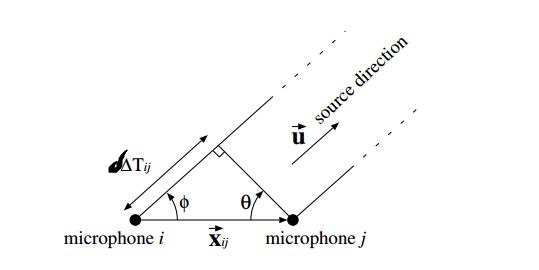
\includegraphics[width= \textwidth]{d.jpg}
\caption{ \cite {17}Graphical depiction of the direction calculating methodology.}
\label{d:logo}
\end{figure}

\paragraph{}
The figure \ref{d:logo} shows the calculation of the angle between the line connecting the microphones which are i and j and the sound source. Since the distance between microphones are no more than 5 m and this recording position is far away from the sound emitting source, wave fronts can be considered as parallel lines emitted by the sound source. Accuracy of this model will be tested by actual data.

\section{Delimitation of the scope}
\paragraph{}
As the final outcome, my intention is to introduce a low cost elephant detecting and localization system specialized for Asian countries using the sensor equipments made in the Sustainable Computing Research Group at University of Colombo School of Computing.

\begin{flushleft}
\text{This research attempts to:}
\end{flushleft}

\begin{itemize}

\item 	Identify an elephant call in the infrasound range with low latency.
\item 	Localizing an elephant call using the low cost sensors system consisting of a condenser microphone.
\end{itemize}

\newpage
\section{Project Schedule}
\begin{table}[h]
\centering
\begin{tabular}{|m{0.5\textwidth}|m{0.5\textwidth}|} 
\hline
\centering \bf {Task} &  \multicolumn{1}{|c|}{\bf{ Completion Date }}\\
\hline
1.Literature review on the project idea & \multicolumn{1}{|m{0.5\textwidth}|}{ \centering  22/04/2016}\\
\hline
2.Finalize the project proposal and submit & \multicolumn{1}{|m{0.5\textwidth}|}{ \centering  28/04/2016}\\
\hline
3.Collecting data from elephants. & \multicolumn{1}{|m{0.5\textwidth}|}{ \centering  19/05/2016}\\
\hline
4.Getting data for localization. & \multicolumn{1}{|m{0.5\textwidth}|}{ \centering 26/05/2016}\\
\hline
5.Analyzing on collected localization data. & \multicolumn{1}{|m{0.5\textwidth}|}{ \centering  13/06/2016}\\
\hline
6.Analyzing on data collected for pattern recognition & \multicolumn{1}{|m{0.5\textwidth}|}{ \centering  22/06/2016}\\
\hline
7.Preparing for Interim presentation. & \multicolumn{1}{|m{0.5\textwidth}|}{ \centering  18/09/2016}\\
\hline
8.Writing thesis chapters on Introduction and related works on localization. & \multicolumn{1}{|m{0.5\textwidth}|}{ \centering  30/09/2016}\\
\hline
9.Implementation of pattern recognition and localization algorithms. & \multicolumn{1}{|m{0.5\textwidth}|}{ \centering 10/10/2016}\\
\hline
10.Writing thesis chapters on current progress. & \multicolumn{1}{|m{0.5\textwidth}|}{ \centering  20/10/2016}\\
\hline
11.Testing the localization and pattern recognition on real world. & \multicolumn{1}{|m{0.5\textwidth}|}{ \centering  20/11/2016}\\
\hline
12.Drafting the full thesis. & \multicolumn{1}{|m{0.5\textwidth}|}{ \centering  10/12/2016}\\
\hline
13.Finalizing the full thesis. & \multicolumn{1}{|m{0.5\textwidth}|}{ \centering  19/12/2016}\\
\hline
14.Project defense. & \multicolumn{1}{|m{0.5\textwidth}|}{ \centering  02/01/2017}\\
\hline
\end{tabular}
\end{table}

\section{Student's personal statement}

\paragraph{}
As an undergraduate with the opportunity to work on a real-world research problem, it is my wish to utilize my time productively by directing my efforts towards conducting a useful research on a burning and timely problem like the human elephant conflict which is also in line with my interest \& passion.

\newpage
\begin{thebibliography}{1}
\bibitem{1} Berg, J.K. 1983. Vocalizations and associated behaviours of the African elephant Loxodonta africana in captivity. Z. Tierpsychol 63:63-79.
\bibitem{2}Payne, K. 2003. Sources of Social Complexity in the Three Elephant Species. In: Animal Social Complexity: Intelligence, Culture, and Individualized Societies. Ed: Frans B.M. de Waal and Peter L. Tyack. Harvard University Press.
\bibitem{3} Payne, K., Langbauer, Jr., W.R., and Thomas, E. 1986. Infrasonic calls of the Asian elephant (Elephas maximus). Behavioral Ecology and Sociobiology.
\bibitem{4} “Infrasonic Sound", Hyperphysics.phy-astr.gsu.edu, 2016. [Online]. Available: http://hyperphysics.phy-astr.gsu.edu/hbase/sound/infrasound.html. [Accessed: 27- Apr- 2016].
\bibitem{5} Szabo T. L., 1994, “Time domain wave equations for lossy media obeying a frequency power law,” J. Acoust. Soc. Am., 96(1), pp. 491-500.
\bibitem{6} Payne, K., Thompson, M., and Kramer, L. 2003. Elephant calling patterns as indicators of group size and composition: the basis for an acoustic monitoring system. African Journal of Ecology, 41: 99-107
\bibitem{7} "INFILTEC: The Inexpensive Infrasound Monitor Project. - simple microbarograph design for DIY", Infiltec.com, 2016. [Online]. Available: http://www.infiltec.com/Infrasound@home/. [Accessed: 27- Apr- 2016].
\bibitem{8} A. Vedurmudi, J. Goulet, J. Christensen-Dalsgaard, B. Young, R. Williams and J. van Hemmen, "How Internally Coupled Ears Generate Temporal and Amplitude Cues for Sound Localization",Phys. Rev. Lett., vol. 116, no. 2, 2016.
\bibitem{9} ] Larom, D., M. Garstang, K. Payne, R. Raspet \& M. Lindeque. 1997. The influence of surface atmospheric conditions on the range and area reached by animal vocalizations. J. Experimental Biol. 200: 421-431.
\bibitem{10} P. J. Venter and J. J. Hanekom. Automatic detection of african elephant (loxodonta africana) infrasonic vocalisations from recordings. Biosystems engineering.
\bibitem{11} Acoustic Detection of Elephant Presence in Noisy Environments Matthias Zeppelzauer Vienna University of Technology.
\bibitem{12} MUSIC Algorithm", Ptolemy.eecs.berkeley.edu, 2016. [Online]. Available: http://ptolemy.eecs.berkeley.edu/papers/96/dtmf\_ict/www/node5.html. [Accessed: 27- Apr- 2016].
\bibitem{13} Lalith Seneviratne, G. Rossel, W.D.C.. Gunasekera, H.L.P.A. Madanayake, Y.M.S.S. Yapa and G. Doluweera.Elephant Infrasound Calls as a Method for Electronic Elephant Detection.
\bibitem{14} J. E. Piercy, T. F. W. Embleton, L. C. Sutherland, Review of noise propagation in the atmosphere, J. Acoust. Soc. Am. Volume 61, Issue 6, pp. 1403-1418, June 1977.
\bibitem{15} Panasonic Corporation. Panasonic Omnidirectional Back Electret Condenser Microphone Cartidge.[2016].  [Online]. Available: http://industrial.panasonic.com/cdbs/www-data/pdf/ABA5000/ABA5000CE22.pdf. [Accessed: 28- Apr- 2016].
\bibitem{16}"LM358 | General Purpose Amplifier | Operational Amplifier (Op Amp) | Description \& parametrics", Ti.com, 2016. [Online]. Available: http://www.ti.com/product/LM358. [Accessed: 28- Apr- 2016].
\bibitem{17}Jean-Marc Valin, Franc¸ois Michaud, Jean Rouat, Dominic Letourneau LABORIUS - Research Laboratory on Mobile Robotics and Intelligent Systems Department of Electrical Engineering and Computer Engineering Universite´ de Sherbrooke.Robust Sound Source Localization Using a Microphone Array on a Mobile Robot.
\bibitem{18} Richard F. Lyon, Andreas G. Katsiamis, Emmanuel M. Drakakis (2010). "History and Future of Auditory Filter Models"

\end{thebibliography}
\end{document}